% Provenance (never printed): see sources/outline_sources.md (Year 3:
% atmospheric dynamics: vorticity and potential vorticity, Rossby waves,
% baroclinic instability, the general circulation and the Hadley cell).
% Brief: sources/book5/BRIEFS.md, ch. 20. Curves from
% figdata/bachelor-3/rossby_waves.py, eady.py and held_hou.py. Exercise and
% problem values in the Book 5 scratch calculator calc/ch20.py. The waves,
% shears and parcels of the exercises and the problem are invented.
\chapter{Dinamika Atmosfer}\label{ch:b3:atmospheric-dynamics}

Pada peta troposfer bagian atas di musim dingin, arus jet tidak
mengelilingi kutub sebagai cincin yang mulus. Arus itu berliku-liku dalam beberapa gelombang besar mengelilingi belahan bumi,
palung menjangkau ke arah subtropik dan punggung ke arah
kutub, dan di permukaan depresi terbentuk, tumbuh selama beberapa hari, lalu mati di bawahnya.
Gelombang-gelombang itu bergerak perlahan, kadang melawan angin yang membawanya.
Jumlah gelombang, kecepatannya, dan pertumbuhan badai di bawahnya
mengikuti dari satu kuantitas kekal, yaitu vortisitas udara yang dilihat dari angkasa,
dan dari energi yang tersimpan dalam kontras suhu antara daerah tropis
dan kutub.

\begin{recall}
Vortisitas dan sirkulasi dibahas dalam buku fisika. Gelombang Rossby di bagian atas
troposfer, palung dan punggung, siklon ekstratropis, serta
prinsip prakiraan cuaca numerik dijelaskan dalam volume Tahun~2,
pada babnya tentang sistem cuaca. Sel Hadley, sel Ferrel, dan sel kutub
arus jet, angin baratan, serta angin momentum sudut dari sebuah cincin
udara dijelaskan dalam volume Tahun~1, pada babnya tentang sirkulasi umum
atmosfer, dan transpor panas ke kutub pada babnya tentang
radiasi dan transpor panas. Parameter Coriolis $f$, bidang-$\beta$,
jari-jari Rossby dan \omterm{thm:b3:gfd-foundations:thermal-wind}{angin termal} dibahas dalam
Bab~\ref{ch:b3:gfd-foundations}.
\end{recall}

\section{Vortisitas}\label{sec:b3:atmospheric-dynamics:vorticity}

Vortisitas suatu fluida, yaitu rotasi dari kecepatannya, sama dengan dua kali kecepatan
sudut lokalnya. Untuk atmosfer skala besar hanya komponen vertikalnya
yang penting, dan rotasi Bumi ikut menyumbangnya.

\begin{definition}[Vortisitas relatif, planeter dan mutlak]\label{def:b3:atmospheric-dynamics:vorticity-kinds}
Untuk kecepatan horizontal $(u, v)$, \emph{vortisitas
relatif}\index{vortisitas relatif} adalah komponen vertikal dari rotasi
kecepatan relatif terhadap tanah, $\zeta = \partial v/\partial x -
\partial u/\partial y$, bernilai positif untuk rotasi berlawanan arah jarum jam jika dilihat dari atas.
\emph{Vortisitas planeter}\index{vortisitas planeter} adalah komponen vertikal
vortisitas rotasi Bumi, $2\Omega\sin\varphi =
f$. \emph{Vortisitas mutlak}\index{vortisitas mutlak} adalah jumlah keduanya,
$\zeta + f$.
\end{definition}

Di Belahan Bumi Utara depresi, tempat udara berputar berlawanan arah jarum jam,
memiliki $\zeta > 0$ dan disebut siklonik; antisiklon memiliki $\zeta < 0$. Angin
sebesar \qty{15}{m/s} yang berputar pada lingkaran berjari-jari \qty{1000}{km} memiliki $\zeta =
2V/R = \qty{3e-5}{s^{-1}}$ dalam rotasi kaku, sepertiga dari $f$ pada \ang{45}:
bagian planeter biasanya yang lebih besar.

\begin{theorem}[Persamaan vortisitas barotropik]\label{thm:b3:atmospheric-dynamics:bve}
Dalam aliran dua dimensi yang tak kental dan tanpa divergensi horizontal pada
bidang-$\beta$, \omterm{def:b3:atmospheric-dynamics:vorticity-kinds}{vortisitas mutlak} setiap parsel dikekalkan:
\[
\frac{\mathrm D(\zeta + f)}{\mathrm Dt} = 0 ,
\qquad\text{yaitu}\qquad
\frac{\partial\zeta}{\partial t} + u\frac{\partial\zeta}{\partial x} + v\frac{\partial\zeta}{\partial y} + \beta v = 0 .
\]
Inilah \emph{persamaan vortisitas barotropik}\index{persamaan vortisitas barotropik}.
\end{theorem}

\begin{proof}
Persamaan momentum horizontal adalah $\mathrm Du/\mathrm Dt - fv =
-(1/\rho_0)\partial p/\partial x$ dan $\mathrm Dv/\mathrm Dt + fu =
-(1/\rho_0)\partial p/\partial y$. Turunkan persamaan kedua terhadap
$x$, persamaan pertama terhadap $y$, lalu kurangkan: tekanan hilang.
Dengan $\delta = \partial u/\partial x + \partial v/\partial y$, suku
adveksi memberikan $\partial_x(u\,\partial_xv + v\,\partial_yv) -
\partial_y(u\,\partial_xu + v\,\partial_yu) = u\,\partial_x\zeta +
v\,\partial_y\zeta + \zeta\delta$, dan suku Coriolis memberikan $f\delta + \beta
v$. Jadi $\mathrm D\zeta/\mathrm Dt + \beta v = -(\zeta + f)\,\delta$. Untuk
$\delta = 0$, dan karena $\mathrm Df/\mathrm Dt = \beta v$ maka $\mathrm D(\zeta +
f)/\mathrm Dt = 0$.
\end{proof}

Pembuktian tadi juga menghasilkan hukum umumnya, $\mathrm D(\zeta + f)/\mathrm Dt =
-(\zeta + f)\delta$: konvergensi memutar sebuah kolom ke atas, divergensi
memutarnya ke bawah, seperti seorang peluncur yang merapatkan atau membentangkan lengannya. Dalam lapisan yang kedalamannya
berubah, konvergensi terkait dengan peregangan kolom, dan
kuantitas yang kekal menjadi suatu rasio.

\begin{definition}[Vortisitas potensial]\label{def:b3:atmospheric-dynamics:pv}
\emph{Vortisitas potensial}\index{vortisitas potensial} sebuah kolom dari lapisan
homogen dengan kedalaman $h$ adalah $q = (\zeta + f)/h$. Dalam fluida yang berlapis kontinu,
vortisitas potensial Ertel adalah $q = (\vec\omega_a\cdot
\nabla\theta)/\rho$, dengan $\vec\omega_a$ vektor \omterm{def:b3:atmospheric-dynamics:vorticity-kinds}{vortisitas mutlak} dan
$\theta$ suhu potensial.
\end{definition}

\begin{theorem}[Kekekalan vortisitas potensial]\label{thm:b3:atmospheric-dynamics:pv}
Dalam lapisan homogen, hidrostatik dan tak kental dengan kedalaman $h$ yang bervariasi,
yang kecepatan horizontalnya tidak berubah terhadap ketinggian, $\mathrm Dq/\mathrm Dt = 0$
untuk $q = (\zeta + f)/h$.
\end{theorem}

\begin{proof}
Dari pembuktian di atas, $\mathrm D(\zeta + f)/\mathrm Dt = -(\zeta + f)\delta$.
Kekekalan massa dalam sebuah kolom dengan massa jenis seragam memberikan $\mathrm Dh/\mathrm
Dt = -h\delta$. Maka $\mathrm Dq/\mathrm Dt = (1/h)\,\mathrm D(\zeta +
f)/\mathrm Dt - ((\zeta + f)/h^2)\,\mathrm Dh/\mathrm Dt = -(\zeta +
f)\delta/h + (\zeta + f)\delta/h = 0$.
\end{proof}

Bentuk Ertel dikekalkan dengan cara yang sama oleh aliran adiabatik tanpa gesekan
dari fluida berlapis, dengan jarak antara dua permukaan $\theta$ yang
konstan berperan sebagai $h$. Sebuah kolom udara yang melintasi
pegunungan terperas saat naik: \omterm{def:b3:atmospheric-dynamics:vorticity-kinds}{vortisitas mutlaknya} turun, ia
berbelok secara antisiklonik di atas punggungan, dan ia meregang serta berbelok
secara siklonik di sisi bawah angin. Kekekalan
\omterm{def:b3:atmospheric-dynamics:vorticity-kinds}{vortisitas mutlak} atau \omterm{def:b3:atmospheric-dynamics:pv}{vortisitas potensial} adalah mekanisme pemulih bagi gelombang
pada bagian berikutnya, seperti ditunjukkan oleh gambar di bawah ini.

\begin{omfigure}
\begin{tikzpicture}[>=stealth, font=\small, declare function={w(\x)=0.9*sin(\x r);}]
\draw[black!40, dashed] (0,0) -- (12.6,0) node[right, font=\scriptsize] {lintang $\varphi_0$};
\draw[thick, omDef, domain=0:12.566, samples=120] plot (\x, {w(\x)});
\foreach \x in {0.785, 2.356, 3.927, 5.498, 7.069, 8.639, 10.21, 11.78}
  \fill (\x, {w(\x)}) circle (0.06);
% crests: clockwise (anticyclonic), troughs: anticlockwise (cyclonic)
\foreach \x in {1.571, 7.854} {
  \draw[->, omThm, thick] (\x+0.45,{w(\x)+0.05}) arc (0:-300:0.45);
  \node[font=\scriptsize, omThm] at (\x,{w(\x)+0.75}) {$\zeta < 0$};}
\foreach \x in {4.712, 10.996} {
  \draw[->, omMeth, thick] (\x+0.45,{w(\x)-0.05}) arc (0:300:0.45);
  \node[font=\scriptsize, omMeth] at (\x,{w(\x)-0.75}) {$\zeta > 0$};}
\foreach \x in {3.1416, 9.4248} \draw[->, very thick] (\x,0.45) -- (\x,-0.45);
\foreach \x in {6.2832} \draw[->, very thick] (\x,-0.45) -- (\x,0.45);
\draw[->, thick] (8.4,-2.25) -- (6.4,-2.25) node[left, font=\scriptsize] {pola bergerak ke barat};
\draw[->] (0,-2.25) -- (1.4,-2.25) node[right, font=\scriptsize] {timur};
\draw[->] (0,-2.25) -- (0,-1.65) node[above, font=\scriptsize] {utara};
\end{tikzpicture}

\par\smallskip{\small Cara gelombang Rossby bergerak (skematis, Belahan Bumi
Utara). Rangkaian parsel yang diam pada lintang $\varphi_0$ tergeser
menjadi gelombang. Dengan menjaga $\zeta + f$, parsel yang bergerak ke utara, tempat
$f$ lebih besar, memperoleh \omterm{def:b3:atmospheric-dynamics:vorticity-kinds}{vortisitas relatif} searah jarum jam; yang bergerak ke selatan
berlawanan arah jarum jam. Di antara puncak dan lembah di timurnya, aliran terinduksi
mengarah ke selatan, di antara lembah dan puncak di timurnya mengarah ke utara (panah
hitam): simpangan membesar di sebelah barat setiap puncak dan seluruh pola
bergeser ke barat.}\label{fig:b3:atmospheric-dynamics:restoring}
\end{omfigure}

\section{Gelombang Rossby}\label{sec:b3:atmospheric-dynamics:rossby}

Volume Tahun~2 membahas gelombang Rossby di troposfer atas. \omterm{thm:b3:atmospheric-dynamics:bve}{Persamaan
vortisitas barotropik} menjelaskannya. Tulis aliran sebagai angin barat
seragam $U$ ditambah gangguan kecil dengan fungsi arus $\psi'$, sehingga
$u' = -\partial\psi'/\partial y$, $v' = \partial\psi'/\partial x$ dan $\zeta'
= \nabla^2\psi'$.

\begin{theorem}[Dispersi gelombang Rossby]\label{thm:b3:atmospheric-dynamics:rossby}
Gangguan kecil $\psi' \propto \mathrm e^{\mathrm i(kx + ly - \omega t)}$
dari angin barat seragam $U$ pada bidang-$\beta$ memenuhi
\emph{relasi dispersi gelombang Rossby}\index{relasi dispersi gelombang Rossby}
\[
\omega = Uk - \frac{\beta k}{k^2 + l^2} .
\]
Kecepatan fase ke timurnya adalah $c = \omega/k = U - \beta/K^2$, dengan $K^2 =
k^2 + l^2$, dan kecepatan grup ke timurnya $c_g = \partial\omega/\partial
k = U + \beta(k^2 - l^2)/K^4$.
\end{theorem}

\begin{proof}
Dilinearkan terhadap $U$, \omterm{thm:b3:atmospheric-dynamics:bve}{persamaan vortisitas barotropik} berbentuk
$(\partial_t + U\partial_x)\nabla^2\psi' + \beta\,\partial_x\psi' = 0$, dengan
perkalian besaran kecil diabaikan dan $\zeta$ aliran dasar
bernilai nol. Untuk gelombang bidang, $\partial_t \to -\mathrm i\omega$,
$\partial_x \to \mathrm ik$ dan $\nabla^2 \to -K^2$: $(-\mathrm i\omega +
\mathrm iUk)(-K^2) + \mathrm i\beta k = 0$, yaitu $(\omega - Uk)K^2 =
-\beta k$. Diferensiasi $\omega$ terhadap $k$ memberikan $c_g = U -
\beta/K^2 + 2\beta k^2/K^4$, yang sesuai dengan bentuk yang dinyatakan.
\end{proof}

\begin{omfigure}
\begin{tikzpicture}
\begin{groupplot}[group style={group size=2 by 1, horizontal sep=1.7cm},
  width=0.48\linewidth, height=0.46\linewidth, tick label style={font=\scriptsize},
  label style={font=\small}, legend style={font=\scriptsize, draw=none, fill=none}]
\nextgroupplot[xlabel={bilangan gelombang zonal $n$}, ylabel={laju (\unit{m/s})},
  xmin=1, xmax=12, ymin=-40, ymax=60, legend pos=north east, legend cell align=left,
  title={\small \ang{45} LU}]
% computed in figdata/bachelor-3/rossby_waves.py
\addplot[omThm, thick] table[x=n, y=c15] {figdata/out/bachelor-3-rossby_waves-disp.dat};
\addlegendentry{$c$, $U = 15$}
\addplot[omThm, thick, densely dashed] table[x=n, y=cg15] {figdata/out/bachelor-3-rossby_waves-disp.dat};
\addlegendentry{$c_g$, $U = 15$}
\addplot[omDef, thick] table[x=n, y=c0] {figdata/out/bachelor-3-rossby_waves-disp.dat};
\addlegendentry{$c$, $U = 0$}
\addplot[omDef, thick, densely dashed] table[x=n, y=cg0] {figdata/out/bachelor-3-rossby_waves-disp.dat};
\addlegendentry{$c_g$, $U = 0$}
\addplot[black!50, thin, domain=1:12, samples=2, forget plot] {0};
\nextgroupplot[xlabel={lintang (\unit{\degree} LU)}, ylabel={bilangan gelombang stasioner $n_s$},
  xmin=20, xmax=75, ymin=0, ymax=9, legend pos=north east, legend cell align=left]
\addplot[omMeth, thick] table[x=lat, y=n10] {figdata/out/bachelor-3-rossby_waves-stat.dat};
\addplot[omDef, thick] table[x=lat, y=n15] {figdata/out/bachelor-3-rossby_waves-stat.dat};
\addplot[omThm, thick] table[x=lat, y=n20] {figdata/out/bachelor-3-rossby_waves-stat.dat};
\addplot[black, only marks, mark=*, mark size=1.1pt] table[x=lat, y=ns] {figdata/out/bachelor-3-rossby_waves-statobs.dat};
\legend{\qty{10}{m/s}, \qty{15}{m/s}, \qty{20}{m/s}, Januari \qty{300}{hPa}}
\end{groupplot}
\end{tikzpicture}

\par\smallskip{\small Kiri, kecepatan fase ke timur $c$ (garis padat) dan
kecepatan grup $c_g$ (putus-putus) gelombang Rossby dengan $l = 0$ pada \ang{45} LU, terhadap
jumlah gelombang di sepanjang lingkaran lintang, tanpa angin rata-rata (biru)
dan dalam angin barat \qty{15}{m/s} (merah): gelombang panjang bergerak ke barat, yang pendek
terbawa ke timur, dan $c_g > c$. Kanan, bilangan gelombang stasioner untuk
angin barat seragam 10, 15 dan \qty{20}{m/s}, serta untuk
angin \omterm{def:b3:atmospheric-dynamics:eddy}{rata-rata zonal} Januari pada \qty{300}{hPa} di setiap lintang (titik-titik, NCEP--NCAR
Reanalysis~1, 1991--2020).}\label{fig:b3:atmospheric-dynamics:rossby}
\end{omfigure}
% ledger: data:b5-ncep-uwnd, geod5:grs80-defining, earth:Rmean

Relatif terhadap udara, gelombang selalu bergerak ke barat, makin panjang
gelombangnya, makin cepat geraknya. Angin barat membawa gelombang pendek ke timur; yang panjang
tidak dapat dibawanya, dan gelombang itu hanyut ke barat melawan angin. Di antara keduanya,
ada satu panjang yang diam di tempat.

\begin{proposition}[Gelombang Rossby stasioner]\label{prop:b3:atmospheric-dynamics:stationary}
Pada angin barat $U > 0$, gelombang tanpa struktur meridional ($l = 0$) bersifat stasioner
jika panjang gelombangnya ialah \emph{panjang gelombang Rossby
stasioner}\index{panjang gelombang Rossby stasioner} $\lambda_s =
2\pi\sqrt{U/\beta}$. Di sepanjang lingkaran lintang $\varphi$, ini berupa bilangan bulat
gelombang yang mendekati $n_s = \sqrt{2\Omega a\cos^3\varphi/U}$.
\end{proposition}

\begin{proof}
$c = 0$ saat $k^2 = \beta/U$, sehingga $\lambda_s = 2\pi/k = 2\pi\sqrt{U/\beta}$.
Lingkaran itu panjangnya $2\pi a\cos\varphi$, sehingga $n_s = a\cos\varphi\,k =
a\cos\varphi\sqrt{2\Omega\cos\varphi/(aU)} = \sqrt{2\Omega a\cos^3\varphi/U}$.
\end{proof}

Pada \ang{45}~LU dalam angin barat sebesar \qty{15}{m/s}, dengan $\beta =
\qty{1.62e-11}{m^{-1}.s^{-1}}$, $\lambda_s = \qty{6050}{km}$ dan $n_s =
4.7$: empat atau lima gelombang mengelilingi belahan bumi. Dengan
\omterm{def:b3:atmospheric-dynamics:eddy}{rata-rata zonal} angin Januari pada \qty{300}{hPa} sekitar \qty{21}{m/s} di \ang{45}~LU, $n_s$ kira-kira
empat dari \ang{35} sampai \ang{55}~LU, dan menurun ke arah kutub. Kecepatan grup
gelombang dengan $l = 0$ melebihi kecepatan fasenya sebesar $2\beta/k^2$: energi
bergerak lebih dulu daripada gelombang, sehingga gangguan yang dimulai di satu tempat membentuk lembah dan punggung baru
di hilirnya, beberapa hari kemudian dan terpaut ribuan kilometer
ke timur, sementara pola itu sendiri hampir tidak bergerak. Pegunungan serta
kontras suhu antara benua dan samudra memicu gelombang stasioner
jenis yang persis sama, melalui peregangan dan pemampatan
\omterm{def:b3:atmospheric-dynamics:pv}{vortisitas potensial}.
% ledger: geod5:grs80-defining, earth:Rmean, data:b5-ncep-uwnd (values in figdata/bachelor-3/rossby_waves.py)


\section{Ketidakstabilan baroklinik}\label{sec:b3:atmospheric-dynamics:baroclinic}

Gelombang pada subbab sebelumnya bersifat netral: tidak tumbuh maupun meluruh.
Badai di lintang menengah tumbuh, dan mengambil energinya dari
kontras suhu yang dinyatakan oleh \omterm{thm:b3:gfd-foundations:thermal-wind}{angin termal}.

\begin{definition}[Energi potensial tersedia]\label{def:b3:atmospheric-dynamics:ape}
Yang disebut \emph{energi potensial tersedia}\index{energi potensial tersedia} dari
suatu fluida terstratifikasi ialah selisih antara energi potensial totalnya
(gravitasi dan internal) dan energi potensial total terkecil yang
dapat dicapainya melalui penataan ulang massa secara adiabatik, yakni keadaan
permukaan bersuhu potensial tetap, atau massa jenis potensial tetap, berupa
bidang mendatar.
\end{definition}

Fluida dengan isentrop mendatar tidak memilikinya, betapa pun besar energi potensial
yang dikandungnya; fluida yang isentropnya miring, hangat dan ringan di satu sisi, dingin
dan padat di sisi lain, dapat melepaskan sebagian dengan membiarkan isentropnya merosot. Pertukaran
dua parsel menunjukkan caranya. Ambil parsel hangat yang rendah di sisi ekuator dan
parsel dingin yang tinggi di sisi kutub, keduanya pada isentrop yang sama dalam
atmosfer stabil yang isentropnya naik ke arah kutub. Menukar keduanya sepanjang
isentrop tidak mengubah apa pun. Menukar keduanya sepanjang lintasan yang lebih landai daripada
isentrop membawa parsel hangat naik dan ke arah kutub, ke udara yang lebih dingin daripada
dirinya sendiri, dan parsel dingin turun ke arah ekuator menuju udara yang lebih hangat:
parsel hangat naik, yang dingin tenggelam, pusat massa turun, dan energi kinetik
dilepaskan. Lintasan di dalam baji antara bidang mendatar dan
isentrop melepaskan energi; \omterm{def:b3:atmospheric-dynamics:eddy}{eddy} di lintang menengah ialah pertukaran
seperti itu, yang memindahkan panas ke arah kutub dan ke atas.

\begin{definition}[Ketidakstabilan baroklinik]\label{def:b3:atmospheric-dynamics:baroclinic-instability}
Yang disebut \emph{ketidakstabilan baroklinik}\index{ketidakstabilan baroklinik} ialah
ketidakstabilan aliran berotasi dan terstratifikasi dalam keseimbangan \omterm{thm:b3:gfd-foundations:thermal-wind}{angin termal}, melalui
gangguan tumbuh dengan mengubah \omterm{def:b3:atmospheric-dynamics:ape}{energi potensial tersedia} dari
isentrop yang miring menjadi energi kinetik gangguan itu sendiri.
\end{definition}

\begin{definition}[Model Eady]\label{def:b3:atmospheric-dynamics:eady}
Yang disebut \emph{model Eady}\index{model Eady} ialah fluida Boussinesq pada
bidang-$f$ di antara dua permukaan mendatar yang kaku pada $z = 0$ dan $z = H$, dengan
\omterm{def:b3:gfd-foundations:buoyancy}{frekuensi daya apung} seragam $N$ dan angin barat yang bertambah secara linear
terhadap ketinggian, $U = \Lambda z$, dalam keseimbangan \omterm{thm:b3:gfd-foundations:thermal-wind}{angin termal} dengan penurunan suhu
seragam ke arah kutub; gangguannya mematuhi
persamaan kuasi-geostrofik.
\end{definition}

\begin{theorem}[Laju pertumbuhan Eady]\label{thm:b3:atmospheric-dynamics:eady}
Pada \omterm{def:b3:atmospheric-dynamics:eady}{model Eady}, gangguan $\propto \mathrm e^{\mathrm ik(x - ct)}$
dengan $\mu = kL_d$, $L_d = NH/f$, tumbuh secara eksponensial bila $\mu < \mu_c =
2.40$, dengan laju
\[
\sigma = \frac{f\Lambda}{N}\left[\left(\coth\frac{\mu}{2} - \frac{\mu}{2}\right)\left(\frac{\mu}{2} - \tanh\frac{\mu}{2}\right)\right]^{1/2} .
\]
Gangguan yang paling cepat tumbuh memiliki $\mu = 1.61$, panjang gelombangnya $2\pi L_d/1.61
\approx 3.9\,L_d$, dan tumbuh dengan laju $\sigma_{\max} = 0.31\,f\Lambda/N$.
\end{theorem}
\admitted

Laju pertumbuhan hanya bergantung pada geseran dan stratifikasi, melalui
$f\Lambda/N$, dan ukuran yang disukai hanya pada jari-jari Rossby. Untuk
rata-rata Januari pada \ang{45}~LU, angin bertambah sebesar \qty{17.2}{m/s} antara
\qty{850}{hPa} dan \qty{250}{hPa}, berjarak sekitar \qty{8.9}{km} dalam
atmosfer standar, geseran sebesar \qty{1.9e-3}{s^{-1}}; dengan rata-rata
troposfer $N = \qty{0.0113}{s^{-1}}$ dan $H = \qty{11}{km}$, $L_d =
\qty{1210}{km}$, gangguan tercepat memiliki panjang gelombang \qty{4700}{km}
dan tumbuh sebesar faktor $e$ dalam \num{2.1}~hari. Gangguan yang lebih pendek daripada
\qty{3200}{km} tidak tumbuh sama sekali. Inilah ukuran dan waktu tumbuh
dari depresi pada peta cuaca.
% ledger: data:b5-ncep-uwnd, nasa:grc-atmos (values in figdata/bachelor-3/eady.py)

\begin{omfigure}
\begin{minipage}[c]{0.52\linewidth}\centering
\begin{tikzpicture}
\begin{axis}[width=\linewidth, height=0.85\linewidth, xmin=2, xmax=16, ymin=0, ymax=0.55,
  xlabel={panjang gelombang (\qty{1000}{km})}, ylabel={laju pertumbuhan (hari$^{-1}$)},
  tick label style={font=\scriptsize}, label style={font=\small}]
% computed in figdata/bachelor-3/eady.py
\addplot[omThm, thick] table[x expr=\thisrow{lam}/1000, y=sday] {figdata/out/bachelor-3-eady-curve.dat};
\addplot[only marks, mark=*, mark size=1.6pt] coordinates {(4.721,0.4701)};
\node[font=\scriptsize, anchor=west] at (axis cs:5.0,0.49) {\qty{4700}{km}: waktu $e$-lipat \qty{2.1}{d}};
\addplot[black!50, densely dashed] coordinates {(3.160,0) (3.160,0.55)};
\node[font=\scriptsize, anchor=west, black!60] at (axis cs:3.25,0.04) {batas potong};
\end{axis}
\end{tikzpicture}
\end{minipage}\hfill
\begin{minipage}[c]{0.44\linewidth}\centering
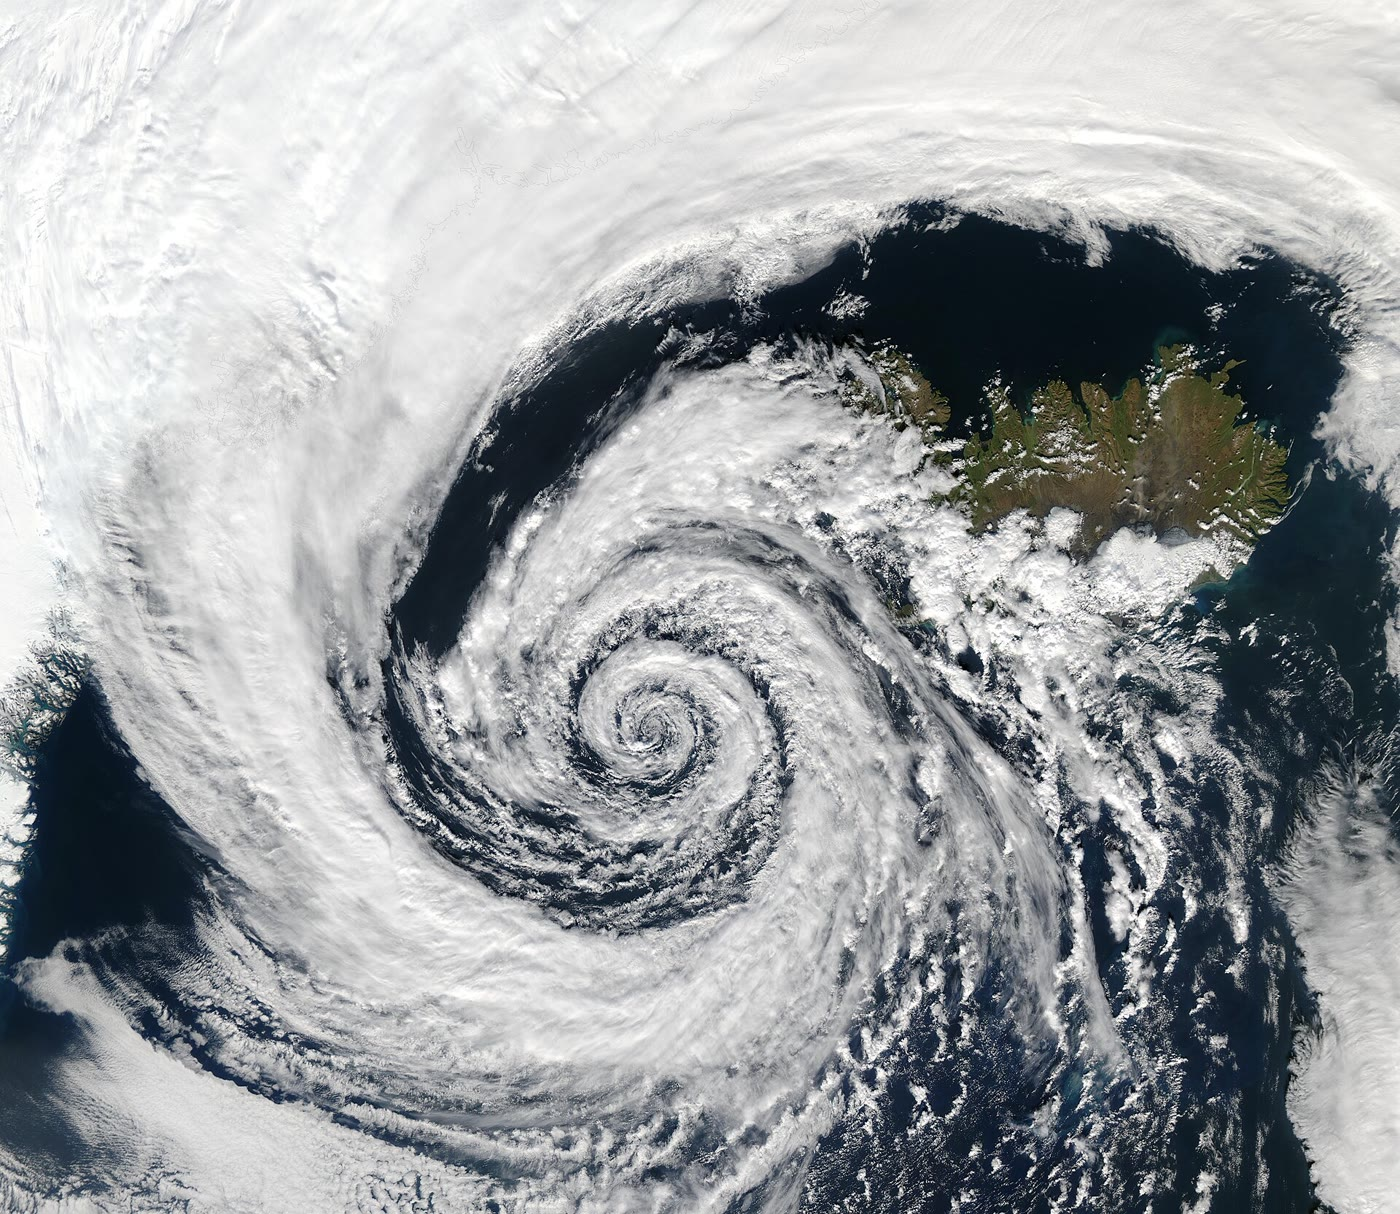
\includegraphics[width=\linewidth]{images/book5/b3-iceland-low.jpg}
\end{minipage}

\par\smallskip{\small Kiri, laju pertumbuhan Eady terhadap panjang gelombang untuk
geseran \omterm{def:b3:atmospheric-dynamics:eddy}{rata-rata zonal} Januari pada \ang{45}~LU (NCEP--NCAR Reanalysis~1,
1991--2020), stratifikasi troposfer rata-rata dan $H = \qty{11}{km}$:
tidak ada pertumbuhan di bawah \qty{3200}{km}, pertumbuhan tercepat di dekat \qty{4700}{km}. Kanan, depresi
dalam tahap dewasa di lepas pesisir barat daya Islandia, 4
September 2003, awannya terpilin membentuk spiral berlawanan arah jarum jam di sekitar
pusat tekanan rendah itu (NASA/GSFC, MODIS Rapid Response Team,
domain publik)}\label{fig:b3:atmospheric-dynamics:eady}
\end{omfigure}
% ledger: data:b5-ncep-uwnd, nasa:grc-atmos, photo:b3-iceland-low

Siklon ekstratropis pada volume Tahun 2 adalah sisi permukaan dari
gelombang \omterm{def:b3:gfd-foundations:baroclinic}{baroklinik} yang sedang tumbuh: sektor hangatnya membawa udara hangat ke arah kutub dan
ke atas, udara dingin di belakangnya meluncur ke arah khatulistiwa dan ke bawah, dan palung di atas
miring ke barat seiring bertambahnya ketinggian, sebagaimana dituntut oleh pelepasan \omterm{def:b3:atmospheric-dynamics:ape}{energi
potensial tersedia}.

\section{Sirkulasi umum}\label{sec:b3:atmospheric-dynamics:general-circulation}

Sirkulasi umum dideskripsikan dengan merata-ratakan sepanjang lingkaran lintang,
dan apa yang ditinggalkan oleh rata-rata itu sama pentingnya dengan apa yang dipertahankannya.

\begin{definition}[Rata-rata zonal dan eddy]\label{def:b3:atmospheric-dynamics:eddy}
Yang disebut \emph{rata-rata zonal}\index{rata-rata zonal} dari suatu besaran $A$ ialah rata-ratanya
sepanjang lingkaran lintang pada ketinggian atau tekanan tetap, $[A] =
(1/2\pi)\int_0^{2\pi} A\,\mathrm d\lambda$. Simpangan $A^* = A - [A]$
adalah bagian eddy-nya; \emph{eddy}\index{eddy (atmosfer)} atmosfer ialah setiap
simpangan aliran dari rata-rata zonalnya: gelombang
berjalan, gelombang stasioner, siklon, dan antisiklon.
\end{definition}

\omterm{def:b3:atmospheric-dynamics:eddy}{Rata-rata zonal} dari suatu hasil kali terbagi dua: $[vT] = [v][T] + [v^*T^*]$. Suku
pertama adalah transpor oleh sirkulasi meridional rata-rata, yaitu sel-sel
pada volume Tahun 1; suku kedua adalah transpor oleh \omterm{def:b3:atmospheric-dynamics:eddy}{eddy}. Di
lintang tengah, angin meridional rata-rata lemah dan suku \omterm{def:b3:atmospheric-dynamics:eddy}{eddy}
mendominasi: udara yang bergerak ke arah kutub lebih hangat daripada udara yang bergerak ke arah khatulistiwa pada
lintang yang sama, seperti pada gambar di bawah, dan $[v^*T^*] > 0$. \omterm{def:b3:atmospheric-dynamics:eddy}{Eddy} juga
membawa momentum angin barat, $[u^*v^*]$, dari subtropik ke lintang
arus jet, itulah sebabnya arus jet dan angin baratan di permukaan
dipertahankan melawan gesekan. Sel Ferrel pada volume Tahun 1 adalah
sirkulasi meridional rata-rata yang dipaksa oleh transpor \omterm{def:b3:atmospheric-dynamics:eddy}{eddy} ini.

\begin{omfigure}
\begin{tikzpicture}[>=stealth, font=\small, declare function={s(\x)=0.9*sin(\x r); t(\x)=0.9*sin((\x+1.0) r);}]
\draw[thick, black, domain=0:12.566, samples=120] plot (\x, {s(\x)});
\draw[omThm, thick, densely dashed, domain=0:12.566, samples=120] plot (\x, {t(\x)-0.15});
\foreach \x in {0.3, 6.58} {\draw[->, omThm, very thick] (\x,-1.1) -- (\x,1.15)
  node[above, font=\scriptsize] {hangat};}
\foreach \x in {3.45, 9.73} {\draw[->, omDef, very thick] (\x,1.1) -- (\x,-1.15)
  node[below, font=\scriptsize] {dingin};}
\node[font=\scriptsize, anchor=west] at (12.7,{s(12.566)}) {garis alir};
\node[font=\scriptsize, anchor=west, omThm] at (12.7,{t(12.566)-0.15}) {isoterm};
\draw[->] (-1.6,-1.1) -- (-0.6,-1.1) node[below, font=\scriptsize] {timur};
\draw[->] (-1.6,-1.1) -- (-1.6,-0.1) node[above, font=\scriptsize] {utara};
\node[font=\scriptsize] at (6.3,-1.95) {udara dingin di utara, hangat di selatan};
\end{tikzpicture}

\par\smallskip{\small Gelombang \omterm{def:b3:gfd-foundations:baroclinic}{baroklinik} yang sedang tumbuh dalam tampak atas (skematik,
Belahan Bumi Utara, aliran barat). Isoterm (putus-putus) tertinggal dari
garis alir sejauh seperempat panjang gelombang atau kurang, sehingga udara yang bergerak ke utara (panah
merah) lebih hangat daripada udara yang bergerak ke selatan pada lintang yang sama (biru):
gelombang itu membawa panas ke arah kutub, $[v^*T^*] >
0$.}\label{fig:b3:atmospheric-dynamics:heatflux}
\end{omfigure}

Di daerah tropis \omterm{def:b3:atmospheric-dynamics:eddy}{eddy} lemah dan sirkulasi rata-rata membawa panas
ke arah kutub, yaitu sel Hadley. Volume Tahun 1 menemukan bahwa udara yang meninggalkan
khatulistiwa dalam keadaan diam dan mempertahankan momentum sudutnya akan berhembus dengan kecepatan ratusan
meter per detik pada \ang{40}, dan tidak menjelaskan mengapa sel berakhir dekat
\ang{30}. Model sederhana memberikan jawabannya.

\begin{definition}[Momentum sudut atmosfer; model Held--Hou]\label{def:b3:atmospheric-dynamics:held-hou}
Yang disebut \emph{momentum sudut atmosfer}\index{momentum sudut atmosfer}
per satuan massa terhadap sumbu Bumi adalah $M = (\Omega a\cos\varphi +
u)\,a\cos\varphi$, untuk angin $u$ yang bertiup ke timur pada lintang $\varphi$. Yang
disebut \emph{model Held--Hou}\index{model Held--Hou} untuk sel Hadley adalah
sirkulasi aksisimetris, tunak, dari atmosfer Boussinesq kering berkedalaman
$H$, dipanaskan dengan relaksasi menuju suhu potensial
kesetimbangan radiatif $\theta_E/\theta_0 = 1 + \Delta/3 - \Delta\sin^2\varphi$; cabang atas
mengonservasi $M$, cabang bawahnya hampir tanpa angin, dan
aliran berada dalam keseimbangan \omterm{thm:b3:gfd-foundations:thermal-wind}{angin termal}.
\end{definition}

\begin{theorem}[Luas sel Hadley]\label{thm:b3:atmospheric-dynamics:held-hou}
Dalam batas sudut kecil, sel Held--Hou mencapai lintang
\[
\varphi_H = \left(\frac{5\,gH\Delta}{3\,\Omega^2a^2}\right)^{1/2}
\]
di setiap belahan bumi, dan angin pada cabang atasnya adalah $u_M = \Omega
a\varphi^2$.
\end{theorem}

\begin{proof}
Untuk $\varphi$ kecil, $\cos\varphi \approx 1$ dan udara yang meninggalkan khatulistiwa dalam
keadaan diam dengan $M = \Omega a^2$ memiliki $u_M = \Omega a(1 - \cos^2\varphi)/\cos\varphi
\approx \Omega a\varphi^2$. Dengan $f \approx 2\Omega\varphi$, $y = a\varphi$,
tidak ada angin di permukaan dan \omterm{thm:b3:gfd-foundations:thermal-wind}{angin termal} dalam bentuk Boussinesq-nya di atas
kedalaman $H$, $2\Omega\varphi\,u_M/H = -(g/a\theta_0)\,\partial\theta_M/
\partial\varphi$, dengan $\theta_M$ adalah rata-rata vertikal dari $\theta$ dalam
sel. Maka $\partial(\theta_M/\theta_0)/\partial\varphi = -2\Omega^2a^2
\varphi^3/(gH)$ dan $\theta_M/\theta_0 = A - K\varphi^4$, $K = \Omega^2a^2/
(2gH)$. Di dalam sel, sirkulasi memindahkan panas tetapi tidak menciptakan maupun
memusnahkannya, sehingga sel memiliki suhu rata-rata yang sama dengan
kesetimbangan radiatif: $\int_0^{\varphi_H}\theta_M\,\mathrm d\varphi = \int_0^{\varphi_H}
\theta_E\,\mathrm d\varphi$. Pada tepinya suhu bersifat kontinu:
$\theta_M(\varphi_H) = \theta_E(\varphi_H)$. Dengan $\theta_E/\theta_0 \approx
B - \Delta\varphi^2$, $B = 1 + \Delta/3$, syarat pertama memberikan $A - B =
K\varphi_H^4/5 - \Delta\varphi_H^2/3$, syarat kedua $A - B = K\varphi_H^4 -
\Delta\varphi_H^2$. Dengan mengurangkan, $(4/5)K\varphi_H^4 = (2/3)\Delta
\varphi_H^2$, maka $\varphi_H^2 = 5\Delta/(6K) = 5gH\Delta/(3\Omega^2a^2)$.
\end{proof}

Sel berakhir di tempat suhu yang diwajibkan oleh kekekalan momentum sudut
bertemu dengan kesetimbangan radiatif; di luar itu, atmosfer harus
lebih dingin daripada yang ditentukan radiasi. Model ini memiliki dua parameter yang
tidak teramati secara langsung. Untuk $H = \qty{15}{km}$ dan $\Delta$ antara $1/6$ dan
$1/3$, dipilih sebagai ilustrasi, $\varphi_H$ adalah \ang{25} sampai \ang{35}. Sel
yang teramati, dibaca dari angin meridional \omterm{def:b3:atmospheric-dynamics:eddy}{rata-rata zonal}, berakhir di
\ang{33.3}~LU dan \ang{32.5}~LS dalam rata-rata tahunan, dan sel musim dingin,
yang kuat, pada \ang{30.8}~LU pada Desember--Februari dan \ang{29.1}~LS pada
Juni--Agustus. Yang penting adalah skalanya: sel yang melebar seiring
troposfer yang lebih dalam dan kontras pemanasan yang lebih kuat, dan menyempit pada
planet yang berotasi lebih cepat. Angin atas model, $u_M =
\qty{88}{m/s}$ pada tepinya untuk $\Delta = 1/6$, adalah dua kali arus jet yang teramati:
\omterm{def:b3:atmospheric-dynamics:eddy}{eddy} menyerap kelebihan itu.
% ledger: geod5:grs80-defining, earth:Rmean, data:b5-ncep-vwnd (values in figdata/bachelor-3/held_hou.py)

\begin{omfigure}
\begin{tikzpicture}
\begin{groupplot}[group style={group size=2 by 1, horizontal sep=1.7cm},
  width=0.48\linewidth, height=0.44\linewidth, tick label style={font=\scriptsize},
  label style={font=\small}, legend style={font=\scriptsize, draw=none, fill=none}]
\nextgroupplot[xlabel={lintang (\unit{\degree})}, ylabel={$100\,(\theta/\theta_0 - 1)$},
  xmin=0, xmax=60, ymin=-30, ymax=15, legend pos=south west, legend cell align=left,
  title={\small $\Delta = 1/3$, $H = \qty{15}{km}$}]
% computed in figdata/bachelor-3/held_hou.py
\addplot[omDef, thick] table[x=phi, y=thE] {figdata/out/bachelor-3-held_hou-theta-3.dat};
\addplot[omThm, thick, unbounded coords=jump] table[x=phi, y=thM] {figdata/out/bachelor-3-held_hou-theta-3.dat};
\addplot[black!50, densely dashed, forget plot] coordinates {(35.26,-30) (35.26,15)};
\node[font=\scriptsize, anchor=south west] at (axis cs:35.6,7) {$\varphi_H$};
\legend{$\theta_E$, $\theta_M$}
\nextgroupplot[xlabel={lintang (\unit{\degree})}, ylabel={$\psi$ pada \qty{500}{hPa} ($10^{10}$\,\unit{kg/s})},
  xmin=-60, xmax=60, ymin=-25, ymax=25, xtick={-60,-30,0,30,60}, legend pos=south west,
  legend cell align=left]
\addplot[black!50, thin, domain=-60:60, samples=2, forget plot] {0};
\addplot[black, thick] table[x=lat, y=ann] {figdata/out/bachelor-3-held_hou-psi.dat};
\addplot[omDef, thick] table[x=lat, y=djf] {figdata/out/bachelor-3-held_hou-psi.dat};
\addplot[omThm, thick] table[x=lat, y=jja] {figdata/out/bachelor-3-held_hou-psi.dat};
\legend{tahunan, Desember--Februari, Juni--Agustus}
\end{groupplot}
\end{tikzpicture}

\par\smallskip{\small Kiri, konstruksi Held--Hou: suhu sel (merah) yang
mengawetkan momentum sudut bertemu kesetimbangan radiatif
(biru) pada $\varphi_H = \ang{35}$, dengan luas yang sama di antara
kurva di dalam sel. Kanan, fungsi aliran massa meridional rata-rata pada
\qty{500}{hPa} dari angin meridional \omterm{def:b3:atmospheric-dynamics:eddy}{rata-rata zonal} (NCEP--NCAR
Reanalysis~1, 1991--2020; positif di mana udara di atas \qty{500}{hPa}
bergerak ke utara): sel belahan bumi musim dingin yang kuat
membentang melintasi khatulistiwa, dan sel-sel berakhir dekat
\ang{30}.}\label{fig:b3:atmospheric-dynamics:held-hou}
\end{omfigure}
% ledger: data:b5-ncep-vwnd

\begin{history}[Dari gelombang panjang ke prakiraan terkomputasi pertama]
Pada 1939 C.-G.~Rossby dan rekan-rekannya, dalam \emph{Journal of Marine
Research}, berupaya menafsirkan beberapa fenomena cuaca yang tampaknya tidak berkaitan
dari satu sudut pandang tunggal. Terdorong oleh pola cuaca yang
bergerak ke hulu melawan aliran angin barat dominan, Rossby menuliskan
teori terlinearisasi, dengan gangguan skala besar cenderung bergerak ke barat
dan yang lebih kecil ke timur relatif terhadap angin: gelombang dan
bidang-$\beta$ dalam bab ini. Sebelas tahun kemudian J.~G.~Charney,
R.~Fjørtoft dan J.~von~Neumann mengintegrasikan \omterm{thm:b3:atmospheric-dynamics:bve}{persamaan vortisitas barotropik}
secara numerik pada komputer elektronik ENIAC: empat prakiraan masing-masing 24~jam pada
aras \qty{500}{mb}, pada kisi \qty{736}{km}, 8 derajat bujur
pada \ang{45}. Perhitungan setiap prakiraan memakan sekitar 24~jam: mereka
hanya mampu, seperti yang mereka tulis, mengimbangi cuaca.
\end{history}
% ledger: rossby39:paper, jmr20:commentary, charney50:eniac

\section{Latihan}

\begin{exercise}[$\star$]\label{exo:b3:atmospheric-dynamics:1}
(a)~Hitung \omterm{def:b3:atmospheric-dynamics:vorticity-kinds}{vortisitas relatif} dari pusaran dalam rotasi kaku yang berputar
sekali sehari. (b)~Hitung \omterm{def:b3:atmospheric-dynamics:vorticity-kinds}{vortisitas planeter} pada \ang{30} dan \ang{60} LU
($\Omega = \qty{7.292e-5}{rad/s}$) dan bandingkan.
\end{exercise}

\begin{exercise}[$\star$]\label{exo:b3:atmospheric-dynamics:2}
Sebuah parsel tanpa \omterm{def:b3:atmospheric-dynamics:vorticity-kinds}{vortisitas relatif} pada \ang{30} LU bergerak ke \ang{40} LU dalam
aliran tanpa divergensi. Hitung \omterm{def:b3:atmospheric-dynamics:vorticity-kinds}{vortisitas relatifnya} di sana. Apakah ia
siklonik atau antisiklonik?
\end{exercise}

\begin{exercise}[$\star$]\label{exo:b3:atmospheric-dynamics:3}
Pada \ang{45} LU, tanpa angin rata-rata, hitung kecepatan fase gelombang Rossby
dengan panjang gelombang \qty{5000}{km} dan $l = 0$. Ke arah mana ia bergerak?
\end{exercise}

\begin{exercise}[$\star$]\label{exo:b3:atmospheric-dynamics:4}
Pada \ang{60} LU di angin barat \qty{10}{m/s}, hitung $\beta$, panjang
gelombang stasioner dan jumlah gelombang stasioner di sekeliling
lingkaran lintang ($a = \qty{6371}{km}$).
\end{exercise}

\begin{exercise}[$\star\star$]\label{exo:b3:atmospheric-dynamics:5}
Sebuah kolom udara dengan kedalaman \qty{10}{km} tanpa \omterm{def:b3:atmospheric-dynamics:vorticity-kinds}{vortisitas relatif} pada \ang{45}
LU, melintasi pegunungan yang menekannya hingga \qty{8}{km}, lalu sebuah cekungan
tempat kedalamannya \qty{12}{km}. Dengan asumsi ia tetap dekat \ang{45} LU, hitung
\omterm{def:b3:atmospheric-dynamics:vorticity-kinds}{vortisitas relatifnya} di atas pegunungan dan di atas cekungan. Di mana
depresi cenderung terbentuk?
\end{exercise}

\begin{exercise}[$\star\star$]\label{exo:b3:atmospheric-dynamics:6}
Untuk gelombang dengan lima puncak di sekeliling lingkaran \ang{45} LU ($l = 0$) pada
angin barat \qty{15}{m/s}, hitung kecepatan fase dan kecepatan grup.
Berapa lama energi gelombang menempuh \qty{5000}{km} ke timur, dan berapa
lama polanya?
\end{exercise}

\begin{exercise}[$\star\star$]\label{exo:b3:atmospheric-dynamics:7}
Pada \ang{45} LU di angin barat \qty{15}{m/s}, sebuah gelombang terkurung di antara
lintang sehingga $l = \pi/(\qty{6000}{km})$. (a)~Hitung bilangan gelombang
zonal stasioner dan panjang gelombangnya. (b)~Tunjukkan bahwa tidak ada gelombang stasioner untuk
$l = \pi/(\qty{3000}{km})$.
\end{exercise}

\begin{exercise}[$\star\star$]\label{exo:b3:atmospheric-dynamics:8}
Dalam \omterm{def:b3:atmospheric-dynamics:eady}{model Eady} pada \ang{45} LU, $\Lambda = \qty{2e-3}{s^{-1}}$, $N =
\qty{0.012}{s^{-1}}$ dan $H = \qty{10}{km}$. Hitung $L_d$, laju pertumbuhan
dan waktu $e$-folding gangguan yang tumbuh paling cepat, serta
panjang gelombangnya.
\end{exercise}

\begin{exercise}[$\star\star$]\label{exo:b3:atmospheric-dynamics:9}
Sepanjang lingkaran lintang, angin meridional \omterm{def:b3:atmospheric-dynamics:eddy}{eddy} adalah $v^* = V\cos kx$ dan
suhu \omterm{def:b3:atmospheric-dynamics:eddy}{eddy} $T^* = T_0\cos(kx - \delta)$, dengan $V = \qty{10}{m/s}$ dan
$T_0 = \qty{5}{K}$. Hitung $[v^*T^*]$ untuk $\delta = 0$, \ang{60} dan
\ang{90}, serta fluks panas yang bersesuaian $\rho c_p[v^*T^*]$ per
\unit{kg/m^3} udara ($c_p = \qty{1004}{J.kg^{-1}.K^{-1}}$). Susunan mana
yang tidak mengangkut panas?
\end{exercise}

\begin{exercise}[$\star\star\star$]\label{exo:b3:atmospheric-dynamics:10}
Mulai dari \omterm{thm:b3:atmospheric-dynamics:bve}{persamaan vortisitas barotropik}, turunkan \omterm{thm:b3:atmospheric-dynamics:rossby}{relasi dispersi
gelombang Rossby} dalam angin barat yang seragam, dan tunjukkan bahwa
relatif terhadap udara setiap gelombang Rossby bergerak ke barat.
\end{exercise}

\begin{exercise}[$\star\star\star$]\label{exo:b3:atmospheric-dynamics:11}
Dalam \omterm{def:b3:atmospheric-dynamics:held-hou}{model Held--Hou}, ambil $H = \qty{12}{km}$ dan $\Delta = 1/4$. Hitung
$\varphi_H$, angin sudut kecil $u_M$ di tepinya dan
angin momentum sudut eksak di sana, dan bandingkan dengan arus jet subtropik
\qty{44}{m/s} pada \omterm{def:b3:atmospheric-dynamics:eddy}{rata-rata zonal} Januari.
\end{exercise}

\begin{exercise}[$\star\star\star$]\label{exo:b3:atmospheric-dynamics:12}
Dua lapisan udara berbeda suhu potensial sebesar \qty{10}{K} pada
\qty{300}{K}; antarmukanya miring naik ke arah kutub dengan kemiringan $s$
sepanjang pita selebar \qty{4000}{km}, dan $\rho = \qty{0.7}{kg/m^3}$. (a)~Tunjukkan
bahwa membiarkan antarmuka mendatar melepaskan $\rho g' s^2L^2/24$ per satuan
luas, dengan $g' = g\,\Delta\theta/\theta$. (b)~Hitung untuk $s = 10^{-3}$ dan
$2\times10^{-3}$ dan bandingkan dengan energi kinetik angin berkecepatan \qty{15}{m/s}
yang melewati \qty{10}{km} udara yang sama.
\end{exercise}
% ledger: geod5:grs80-defining, earth:Rmean, data:b5-ncep-uwnd

\section{Soal: Gelombang yang diam}

\begin{problem}[{Soal akhir pekan --- vortisitas, gelombang Rossby dan
pertumbuhan gelombang \omterm{def:b3:gfd-foundations:baroclinic}{baroklinik} pada \ang{45} LU}]
\label{pb:b3:atmospheric-dynamics:1}
Aliran barat berkecepatan \qty{15}{m/s} melintasi lintang tengah sebuah
benua rekaan, sepanjang \ang{45} LU. Ambil $\Omega =
\qty{7.292115e-5}{rad/s}$, $a = \qty{6371}{km}$ dan $g = \qty{9.81}{m/s^2}$.
Semua nilai aliran tersebut bersifat rekaan.

\medskip\noindent\textbf{Bagian I --- Parsel udara yang tergeser.}
\begin{enumerate}
\item Sebuah parsel tanpa \omterm{def:b3:atmospheric-dynamics:vorticity-kinds}{vortisitas relatif} pada \ang{45} LU didorong ke
  \ang{50} LU. Hitung $f$ pada kedua lintang dan \omterm{def:b3:atmospheric-dynamics:vorticity-kinds}{vortisitas relatifnya} pada
  \ang{50} LU, jika aliran tanpa divergensi.
\item Bergerak dengan \qty{15}{m/s}, sepanjang jari-jari kelengkungan berapa ia berbelok
  (anggap $\zeta = -V/R$, seluruhnya berasal dari kelengkungan)? Ke arah mana ia berbelok?
\item Jika kolomnya juga menyusut dari \qty{10.0}{km} menjadi \qty{9.5}{km} selama
  perjalanan, berapa \omterm{def:b3:atmospheric-dynamics:vorticity-kinds}{vortisitas relatifnya} pada \ang{50} LU?
\item Jika sebaliknya didorong ke \ang{40} LU tanpa divergensi, berapa \omterm{def:b3:atmospheric-dynamics:vorticity-kinds}{vortisitas relatif}
  yang diperolehnya? Jelaskan mengapa parsel yang tergeser dari lintangnya
  berosilasi di sekitar lintang itu.
\end{enumerate}

\medskip\noindent\textbf{Bagian II --- Gelombang yang merambat.}
\begin{enumerate}[resume]
\item Hitung $\beta$ pada \ang{45} LU dan panjang lingkaran lintang tersebut.
\item Untuk $n = 3$ sampai 8 gelombang mengelilingi lingkaran ($l = 0$), hitung
  panjang gelombang, kecepatan fase, dan kecepatan grup dalam angin barat
  sebesar \qty{15}{m/s}.
\item Gelombang mana yang bergerak ke barat, mana ke timur? Berapa hari yang dibutuhkan gelombang
  $n = 5$ untuk bergerak \qty{1000}{km}?
\item Punggungan di atas bagian barat benua menguat. Di mana, dan setelah
  berapa lama, pengaruh gelombang $n = 6$ akan mencapai sejauh
  \qty{5000}{km} di hilir?
\end{enumerate}

\medskip\noindent\textbf{Bagian III --- Gelombang yang diam.}
\begin{enumerate}[resume]
\item Hitung \omterm{prop:b3:atmospheric-dynamics:stationary}{panjang gelombang Rossby stasioner} dan bilangan gelombang stasioner pada
  \ang{45} LU.
\item Hitung bilangan gelombang stasioner untuk angin barat sebesar 10 dan
  \qty{20}{m/s}. Apa yang terjadi pada gelombang stasioner ketika angin barat
  menguat pada musim dingin?
\item Hitung bilangan gelombang stasioner pada \ang{35} LU dan \ang{55} LU dalam
  angin barat sebesar \qty{15}{m/s}.
\item Gunung-gunung di barat benua menjulang \qty{2}{km} ke dalam
  troposfer setebal \qty{10}{km}. Hitung \omterm{def:b3:atmospheric-dynamics:vorticity-kinds}{vortisitas relatif} kolom
  yang melintasinya tanpa mengubah lintang. Mengapa gunung memaksa
  munculnya gelombang stasioner?
\item Mengapa pola gelombang yang dipaksakan gunung itu diam
  hanya ketika panjang gelombangnya mendekati $\lambda_s$?
\end{enumerate}

\medskip\noindent\textbf{Bagian IV --- Badai yang tumbuh.}
\begin{enumerate}[resume]
\item Angin barat bertambah dari permukaan tanah hingga \qty{10}{km} sebesar
  \qty{25}{m/s}. Hitung geser $\Lambda$, dan gradien suhu ke arah kutub
  yang diimplikasikannya oleh \omterm{thm:b3:gfd-foundations:thermal-wind}{angin termal} pada suhu rata-rata
  \qty{250}{K}.
\item Dengan $N = \qty{0.011}{s^{-1}}$, hitung bilangan Richardson
  $N^2/\Lambda^2$. Apakah aliran tidak stabil terhadap turbulensi geser skala kecil?
\item Hitung jari-jari Rossby $L_d$ untuk $H = \qty{10}{km}$.
\item Hitung panjang gelombang gangguan Eady yang paling cepat tumbuh dan
  jumlah gelombang semacam itu yang mengelilingi lingkaran lintang.
\item Hitung panjang gelombang terpendek yang tumbuh.
\item Hitung laju pertumbuhan $\sigma_{\max}$.
\item Dengan faktor berapa gangguan tumbuh dalam tiga hari?
\item Bandingkan panjang gelombang badai yang tumbuh dengan panjang
  gelombang stasioner pada Bagian~III: mana yang lebih panjang, dan apa implikasinya bagi
  gerak badai relatif terhadap gelombang stasioner?
\item Ke arah mana palung gelombang yang tumbuh miring terhadap ketinggian, dan
  mengapa harus demikian?
\item Berikan waktu $e$-folding dari gangguan Eady yang paling cepat tumbuh.
\end{enumerate}
\end{problem}
% ledger: geod5:grs80-defining, earth:Rmean
